\documentclass[12pt,a4paper]{article}
\usepackage[utf8]{inputenc}
\usepackage{amsmath}
\usepackage{amsfonts}
\usepackage{amssymb}
\usepackage{graphicx}
\usepackage[left=2cm,right=2cm,top=2cm,bottom=2cm]{geometry}

\begin{document}
\par\noindent
HINWEIS:
Zum erzeugen der Diagramme wurde ein Bash Script geschrieben, welches der Abgabe beiliegt. Dieses war nötig, da gnuplot Probleme beim erzeugen vieler Diagramme auf einmal hat, aus dem Grund das dieses vom Terminalsystem abhängig sind. Daher erzeugt das Script buildPlot.sh alle png als auch gnuplot Dateien. Die gnuplot Dateien können aber wie gewohnt geplotet werden.\\
Des Weiteren wurde der Test einmal mit Berechnung über die ganze Matrix durch geführt und einmal die Symmetrieeigenschaften der Matrix ausgenutzt.\\
\section*{Leistungstest mit ganzer Matrix}
\begin{figure}[h!]
\centering
\includegraphics[width=0.8\textwidth]{{WEAK_SCALING_JA.dat}.png}
\end{figure}
\begin{figure}[h!]
\centering
\begin{tabular}{c | c | c | c}
Prozesse & Knoten & Interlines & Zeit in Sekunden \\
1 & 1 & 100 & 37.2353 \\
2 & 1 & 141 & 36.7564 \\
4 & 2 & 200 & 37.3686 \\
8 & 4 & 282 & 39.5706 \\
16 & 4 & 400 & 40.0696 \\
24 & 4 & 490 & 40.0879 \\
64 & 8 & 800 & 39.2513 \\
\end{tabular}
\end{figure}
\par\noindent
Der Graph verhält sich sehr merkwürdig, da der Speedup weder Weak skaliert sondern bei sehr wenigen Prozessen sogar Strong. Die könnte sich erklären lassen, damit, dass die Kommunikation bei über mehrere Rechner verläuft und damit die Daten erst hin und her gesendet werden müssen. 
Dies wird ebenfalls unterstützt dadurch, dass pro Mainboard 2 CPUs verbaut sind und somit die Rechnungen mit zwei Knoten noch auf dem gleichen Mailboard ausgeführt werden. 
\newpage
\begin{figure}[h!]
\centering
\includegraphics[width=0.8\textwidth]{{WEAK_SCALING_GS.dat}.png}
\end{figure}

\begin{figure}[h!]
\centering
\begin{tabular}{c | c | c | c}
Prozesse & Knoten & Interlines & Zeit in Sekunden \\
1 & 1 & 100 & 36.7030\\
2 & 1 & 141 & 71.8596\\
4 & 2 & 200 & 73.0463\\
8 & 4 & 282 & 82.2029\\
16 & 4 & 400 & 76.5996\\
24 & 4 & 490 & 77.1833\\
64 & 8 & 800 & 77.6653\\
\end{tabular}
\end{figure}
\par\noindent
Dieser Verlauf verhält sich nicht äquivalent zu dem Jacobi Verfahren. Allerdings existiert bei beim Jakobi Verfahren keine Pipeline, somit kann es sein, dass hier die Laufzeit deutlich durch das Pipelining verzögert wird.
\newpage
\begin{figure}[h!]
\centering
\includegraphics[width=0.8\textwidth]{{STRONG_SCALING_JA.dat}.png}
\end{figure}
\begin{figure}[h!]
\centering
\begin{tabular}{c | c | c | c}
Prozesse & Knoten & Interlines & Zeit in Sekunden \\
12 & 1 & 960 & 186.6984\\
24 & 2 & 960 & 94.7785\\
48 & 4 & 960 & 49.3370\\
96 & 8 & 960 & 25.8823\\
120 & 10 & 960 & 21.7832\\
240 & 10 & 960 & 16.8659\\
\end{tabular}
\end{figure}
\par\noindent
Bei diesen Messungen tritt wie erwartet das Strong-Scaling auf, allerdings ist auch zu sehen, dass ab einer bestimmten Prozesszahl kaum noch Speedup auftritt. Dies kann sich damit erklären, dass die Kommunikation zwischen den Knoten zu lange dauert, als dass es noch zu einem Speedup kommt.
\newpage
\begin{figure}[h!]
\centering
\includegraphics[width=0.8\textwidth]{{STRONG_SCALING_GS.dat}.png}
\end{figure}
\begin{figure}[h!]
\centering
\begin{tabular}{c | c | c | c}
Prozesse & Knoten & Interlines & Zeit in Sekunden \\
12 & 1 & 960 & 371.0067\\
24 & 2 & 960 & 190.9016\\
48 & 4 & 960 & 96.5915\\
96 & 8 & 960 & 51.3105\\
120 & 10 & 960 & 42.3742\\
240 & 10 & 960 & 31.5057\\
\end{tabular}
\end{figure}
\par\noindent
Auch hier tritt das Strong-Scaling auf, allerdings ist hier wie schon bei Weak-Scaling zu sehen, dass das Gauss Seidel Verfahren deutlich langsamer ist, als das Jacobi Verfahren, was ebenfalls auf eine erhöhte kommunikation zurück führen könnte.
\newpage
\begin{figure}[h!]
\centering
\includegraphics[width=0.8\textwidth]{{COMMUNICATION_A_JA.dat}.png}
\end{figure}
\begin{figure}[h!]
\centering
\begin{tabular}{c | c | c | c}
Prozesse & Knoten & Interlines & Zeit in Sekunden \\
10 & 1 & 200 & 19.8375\\
10 & 2 & 200 & 19.8375\\
10 & 3 & 200 & 22.9522\\
10 & 4 & 200 & 27.3824\\
10 & 6 & 200 & 29.9228\\
10 & 8 & 200 & 30.7260\\
10 & 10 & 200 & 73.8324\\
\end{tabular}
\end{figure}

\begin{figure}[h!]
\centering
\includegraphics[width=0.8\textwidth]{{COMMUNICATION_A_GS.dat}.png}
\end{figure}
\newpage
\begin{figure}[h!]
\centering
\begin{tabular}{c | c | c | c}
Prozesse & Knoten & Interlines & Zeit in Sekunden \\
10 & 1 & 200 & 44.9182\\
10 & 2 & 200 & 48.7818\\
10 & 3 & 200 & 54.1011\\
10 & 4 & 200 & 55.8813\\
10 & 6 & 200 & 55.6212\\
10 & 8 & 200 & 57.5855\\
10 & 10 & 200 & 115.6501\\
\end{tabular}
\end{figure}
\par\noindent
Auf den letzten beiden Diagrammen ist der Tradeoff zwischen der Anzahl der Knoten und den Prozessen zu sehen. Hierbei ist deutlich zu erkennen, dass der Speedup deutlich zu nimmt je weniger Prozesse benutzt werden. Auffällig ist auch, dass bei 10 Prozessen mit 10 Knoten die Laufzeit deutlich zu nimmt.
Dies folgt daraus, dass die Daten zwar bei vielen Prozessen besser auf geteilt werden, aber die Kommunikation zu lange im Vergleich zur Rechnung braucht. Auch hier ist zu erkennen, dass das Gauss Seidel verfahren deutlich langsamer ist als das Jacobi Verfahren.
\newpage
\section*{Leistungstest mit halber Matrix}
Generell gelten alle Aussagen wie bei der Berechnung mit der ganzen Matrix es gibt aber aber ein paar Auffälligkeiten (abgesehen vom deutlichen Speedup).
\begin{figure}[h!]
\centering
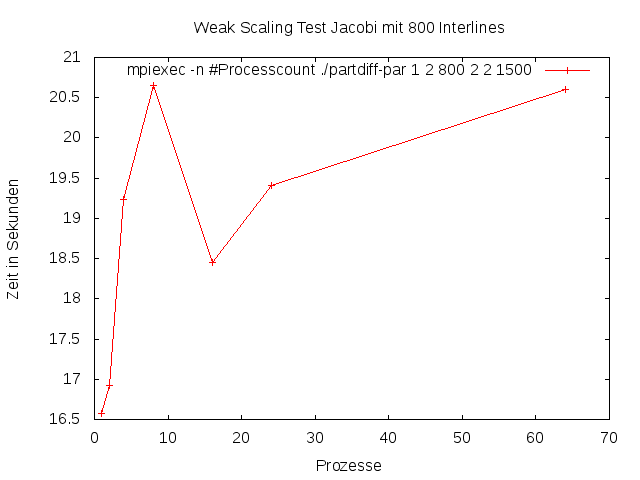
\includegraphics[width=0.8\textwidth]{{halfMatrix/WEAK_SCALING_JA.dat}.png}
\end{figure}
\begin{figure}[h!]
\centering
\begin{tabular}{c | c | c | c}
Prozesse & Knoten & Interlines & Zeit in Sekunden \\
1 & 1 & 100 & 16.5776\\
2 & 1 & 141 & 16.9267\\
4 & 2 & 200 & 19.2339\\
8 & 4 & 282 & 20.6576\\
16 & 4 & 400 & 18.4460\\
24 & 4 & 490 & 19.4137\\
64 & 8 & 800 & 20.6017\\
\end{tabular}
\end{figure}
\par\noindent
Hier ist schon deutlich zu sehen, dass der Speedup nicht äquivalent zu dem mit der ganzen Matrix ist. Des Weiteren ist dieser enormen Schwankungen unterworfen, für die es schwierig ist eine Erklärung zu finden.
\newpage
\begin{figure}[h!]
\centering
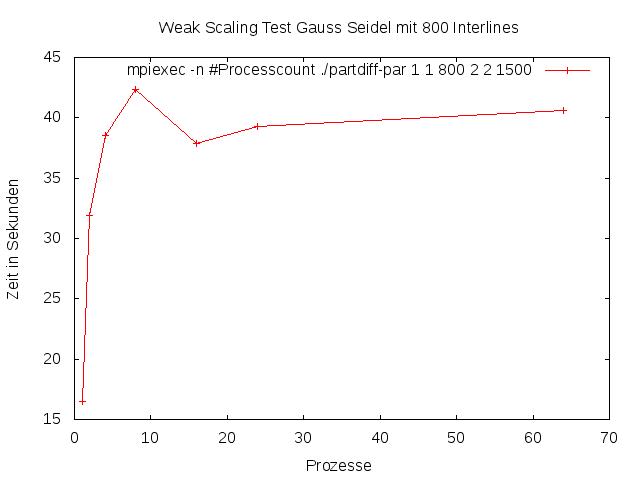
\includegraphics[width=0.8\textwidth]{{halfMatrix/WEAK_SCALING_GS.dat}.png}
\end{figure}
\begin{figure}[h!]
\centering
\begin{tabular}{c | c | c | c}
Prozesse & Knoten & Interlines & Zeit in Sekunden \\
1 & 1 & 100 & 16.5143\\
2 & 1 & 141 & 31.8934\\
4 & 2 & 200 & 38.4988\\
8 & 4 & 282 & 42.3797\\
16 & 4 & 400 & 37.8935\\
24 & 4 & 490 & 39.2747\\
64 & 8 & 800 & 40.6173\\
\end{tabular}
\end{figure}
\par\noindent
Dieses entspricht wieder dem Diagramm wie es bei der ganzen Matrix vorkommt. Auch hier ist der Peek bei 8 Prozessen auf 4 Knoten deutlich zu sehen. Daher gelten hier die gleichen Annahmen wie für die ganze Matrix.
\newpage
\begin{figure}[h!]
\centering
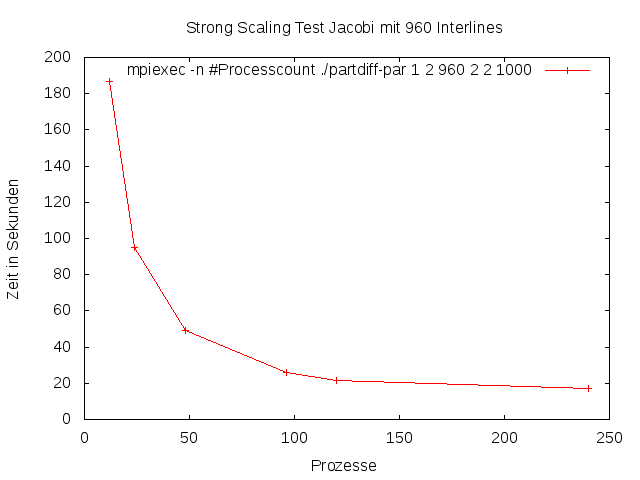
\includegraphics[width=0.8\textwidth]{{halfMatrix/STRONG_SCALING_JA.dat}.png}
\end{figure}
\begin{figure}[h!]
\centering
\begin{tabular}{c | c | c | c}
Prozesse & Knoten & Interlines & Zeit in Sekunden \\
12 & 1 & 960 & 92.5276\\
24 & 2 & 960 & 46.7365\\
48 & 4 & 960 & 23.6457\\
96 & 8 & 960 & 13.1495\\
120 & 10 & 960 & 11.1422\\
240 & 10 & 960 & 8.3299\\
\end{tabular}
\end{figure}
\par\noindent
Auch dies entspricht im wesentlichen dem Diagramm der ganzen Matrix, allerdings mit deutlichem Speedup.
\newpage
\begin{figure}[h!]
\centering
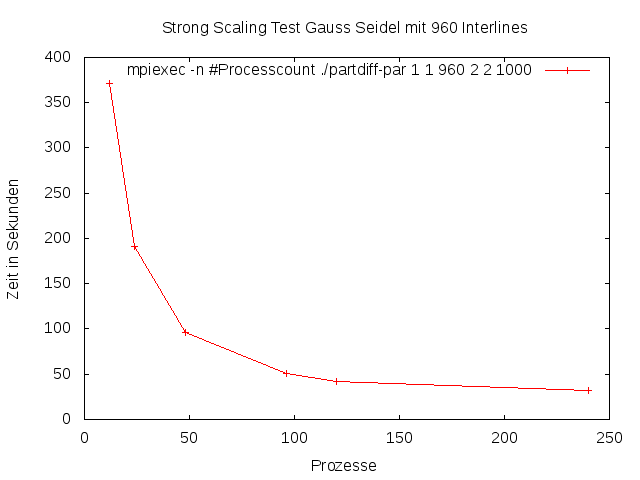
\includegraphics[width=0.8\textwidth]{{halfMatrix/STRONG_SCALING_GS.dat}.png}
\end{figure}
\begin{figure}[h!]
\centering
\begin{tabular}{c | c | c | c}
Prozesse & Knoten & Interlines & Zeit in Sekunden \\
12 & 1 & 960 & 180.0979\\
24 & 2 & 960 & 91.7301\\
48 & 4 & 960 & 47.0823\\
96 & 8 & 960 & 25.3110\\
120 & 10 & 960 & 20.9114\\
240 & 10 & 960 & 15.0807\\
\end{tabular}
\end{figure}
\par\noindent
Auch hier ist der Speedup wie bei der ganzen Matrix. Des Weiteren tritt hier das gleiche Phänomen auf, dass die Gauss Seidel Implementierung deutlich langsamer ist als die Jacobi.
\newpage
\begin{figure}[h!]
\centering
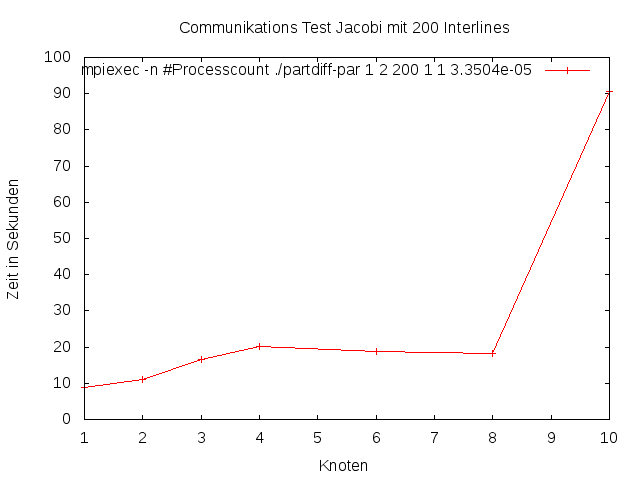
\includegraphics[width=0.8\textwidth]{{halfMatrix/COMMUNICATION_A_JA.dat}.png}
\end{figure}
\begin{figure}[h!]
\centering
\begin{tabular}{c | c | c | c}
Prozesse & Knoten & Interlines & Zeit in Sekunden \\
10 & 1 & 200 & 8.9073\\
10 & 2 & 200 & 11.1802\\
10 & 3 & 200 & 16.4681\\
10 & 4 & 200 & 20.2083\\
10 & 6 & 200 & 18.8340\\
10 & 8 & 200 & 18.2863\\
10 & 10 & 200 & 90.7397\\
\end{tabular}
\end{figure}
\par\noindent
Auch hier ist noch deutlich zu erkennen, dass die Laufzeit zu erst mit steigender Prozessorzahl zu nimmt, dann aber bei 10 Knoten mit 10 Prozessen ebenfalls wie mit der ganzen Matrix einen erheblichen Leistungsverlust aufweist. Des Weiteren ist ein Speedup bei 6 Knoten und 8 Knoten zu sehen, welcher mit 1 Sekunde aber noch im Bereich der Messungenauigkeit liegen könnte.
\newpage
\begin{figure}[h!]
\centering
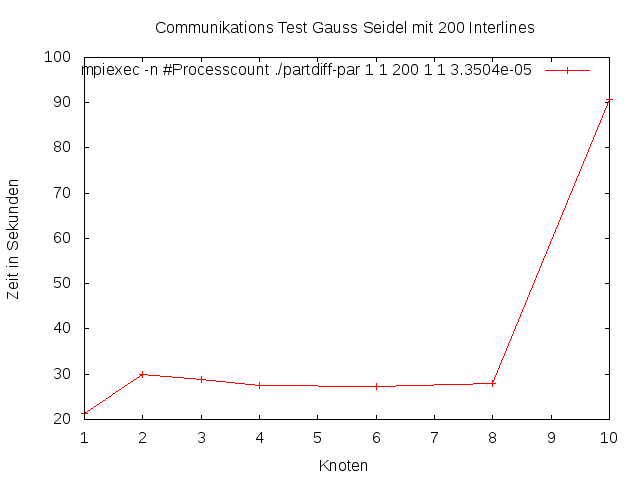
\includegraphics[width=0.8\textwidth]{{halfMatrix/COMMUNICATION_A_GS.dat}.png}
\end{figure}
\begin{figure}[h!]
\centering
\begin{tabular}{c | c | c | c}
Prozesse & Knoten & Interlines & Zeit in Sekunden \\
10 & 1 & 200 & 21.3640\\
10 & 2 & 200 & 29.9315\\
10 & 3 & 200 & 28.8721\\
10 & 4 & 200 & 27.5717\\
10 & 6 & 200 & 27.3327\\
10 & 8 & 200 & 27.8565\\
10 & 10 & 200 & 90.8006\\
\end{tabular}
\end{figure}
\par\noindent
Auch hier ist das Phänomen zu erkennen, dass der Speedup mit steigender Prozessanzahl steigt, dann aber das Programm bei 10 Knoten mit 10 Prozessen einen erheblichen Leistungsverlust hat.
\end{document}